
\section{Models and Implementation}

\subsection{Convolutional Neural Network}

\begin{figure}
    \centering
    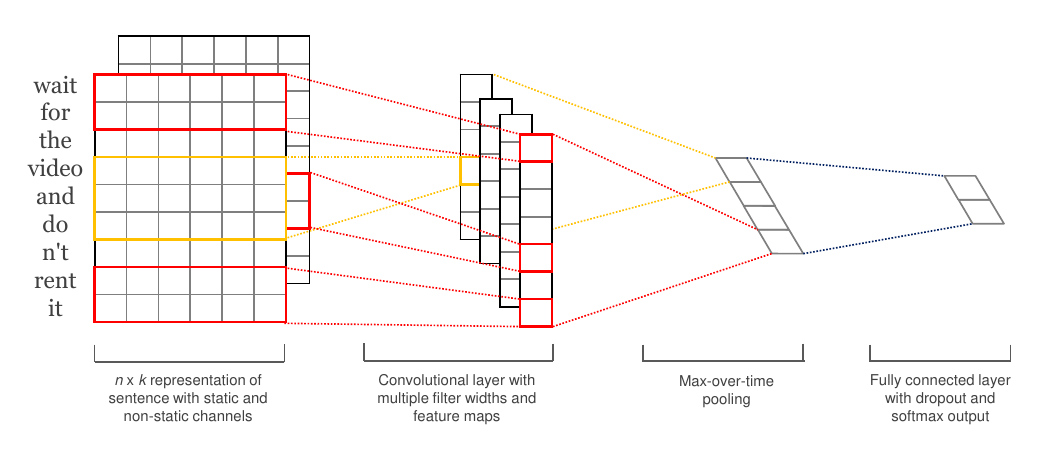
\includegraphics[width=\textwidth]{text_cnn.png}
    \caption{CNN Architecture For Text Classification~\cite{cnn14}}\label{fig:arch}
\end{figure}

The basic structure of the CNN we use can be seen in~\cref{fig:arch} which is
taken directly from~\cite{cnn14}. Every tweet will be split in a sequence of $n$
words $\left(w_1, w_2, \dots, w_n\right)$. For shorter tweets we pad the sequence
with a special pad word $w_{pad}$. Every word $w_i$ is associated with an embedding
vector $\mathbf{x}_{w_i} \in \mathbb{R}^k$.

These embedding vectors can either be static
and come from a pretrained embedding, such as \textit{word2vec}~\cite{word2vec}
or \textit{GloVe}~\cite{glove}, or be dynamically adapted during training.

Each tweet has therefore a representation $\mathbf{X} \in \mathbb{R}^{n \times k}$. Let
$\mathbf{W} \in \mathbb{R}^{h \times k} h \le n$ and
$v_t = \sum_{i = t}^{t + h}\sum_{j = 0}^{k} \mathbf{W}_{i,j} \mathbf{X}_{i,j}$ $\forall 1 \le t \le n - h + 1$.
The resulting vector $\mathbf{v}$ is the convolution of $\mathbf{X}$ and $\mathbf{W}$.
Furthermore let $c_t = f\left(v_t + b\right)$ where $f$ is some non-linear function
and $b \in \mathbb{R}$ a bias term. The resulting vector $\mathbf{c} \in \mathbb{R}^{n - h + 1}$ is called
a feature map.

The feature map $\mathbf{c}$ is then maxpooled which means we select $\hat{c} = \max_{t}\left\{c_t\right\}$.

This process shows how we extract one feature $\hat{c}$ using one filter $\mathbf{W}$.
We use several filters with possibly different heights $h$ in parallel to get
a feature vector $\mathbf{\hat{c}}$, which is then fed into a fully connected
neural network to predict the correct label~\cite{cnn14}~\cite{cnnBlog}.

We based our implementation of the described network on~\cite{cnnBlog} and~\cite{cnnImpl}.
We chose filter lengths $3$, $4$, $5$ and $6$. For each filter length we used
$128$ different filters, resulting in a total of $512$ features.
We initialize the filter parameters and embedding vectors with gaussian
random vectors. We use a dropout rate of $0.5$ for regularization.

\subsection{TF-IDF}

This model is based on the bag of words assumption where each document is
represented by the multiset of words it contains. \textit{TF} stands for
\textit{term freqruency} and measures how often a certain word $w$ appears in
a specific document $d$. Given some document $d$ of length $n$, $d = {\left\{w_i\right\}}_{i = 1}^{n}$
we have $tf\left(w, d\right) = \frac{|\left\{w_i = w | 1 \le i \le n\right\}|}{n}$

\textit{IDF} stands for the \textit{inverse document frequency}
where the \textit{document frequency} measures in how many documents $w$ appears
at least once given some corpus of documents
$\mathcal{C}$. $idf\left(w, \mathcal{C}\right) = \frac{|\mathcal{C}|}{|\left\{d \in \mathcal{C} | w \in d\right\}|}$.
%In order to avoid a division by $0$ on previously unseen terms we add a dummy
%document containing every word and get: $idf\left(w, \mathcal{C}\right) = \frac{|\mathcal{C}| + 1}{|\left\{d \in \mathcal{C} | w \in d\right\}| + 1}$

In its simplest form the \textit{TF-IDF} score of a word $w$ given a document $d$
and corpus $\mathcal{C}$ is $tfidf\left(w, d, \mathcal{C}\right) = tf\left(w, d\right)idf\left(w, \mathcal{C}\right)$.

Using this we can build a sparse feature vector $\mathbf{x}_d \in \mathbb{R}^{|\mathcal{V}|}$
for some document $d$ where $\mathcal{V}$ is the set of all words in the whole
corpus $\mathcal{C}$.

We use these features to train a tree ensemble using gradient boosting~\cite{gradBoost}.

\subsection{GloVe Cluster Features}

Methods such as \textit{GloVe}~\cite{glove} and \textit{word2vec}~\cite{word2vec}
embed words in an euclidean vector space, suggesting that similar words are 
closer together in that space.

Assume we have an embedded vector $x_w \in \mathbb{R}^{m}$ for each word $w$ in our vocabulary.
We cluster these vectors using \textit{k-means} and get a clustering
$c : \mathbb{R}^{m} \rightarrow \left\{1, 2, 3, \dots, k\right\}$.
Given a document $d$ of length $n$, $d = {\left\{w_i\right\}}_{i = 1}^{n}$,
we can construct the following features: $f_j = \frac{|\left\{w \in d | c\left(x_w\right) = j\right\}|}{n}$
for $1 \le j \le k$.

The features $f_j$ represent the normalized histogram of words in the document belonging to
a certain cluster $j$ of words.

When training \textit{GloVe} vectors we used an embedding dimension of $128$ and
trained the model for $10$ epochs.

